\documentclass[14pt]{beamer}
\usetheme{Boadilla}
\usecolortheme{whale}
\setbeamertemplate{navigation symbols}{}
\usepackage{comment}

%\setbeamertemplate{theorems}[numbered]

\usepackage{textcomp}
\usepackage{float}
\usepackage{multirow}
\usepackage{comment}
\usepackage{enumitem}
\usepackage{tikz}
\usepackage{algorithm}
\usepackage{adjustbox}
\usepackage{epstopdf}
\usetikzlibrary{arrows,decorations.pathreplacing,shapes}
\usepackage{amsmath}
\usepackage{multicol}
\usepackage{threeparttable}
\usepackage{mathrsfs}
\usepackage{arydshln}

%\usepackage[UTF8, heading = false, scheme = plain]{ctex}


\usepackage{amsfonts,amsthm,amssymb,amsmath}
\usepackage{graphicx,mathrsfs}
\usepackage{adjustbox}
\usepackage{multirow}
\usepackage{float}
\usepackage{hyperref}
\usepackage{tikz}
\usetikzlibrary{backgrounds}
\usepackage{algorithm}
%\usetikzlibrary{snakes}
\usepackage{subfig}
\usepackage{ragged2e}
\usepackage{framed}
\usepackage{multicol}
\definecolor{shadecolor}{rgb}{0.9,0.9,0.9}

\setbeamerfont{frametitle}{size=\large}


% Setup appearance:


\newcommand{\labelitemi}{$\bullet$}
\newcommand{\BM}{\mathcal{B}} % Brownian motion
\newcommand{\cl}[1]{\lceil{#1}\rceil} % ceiling of a number
\newcommand{\R}{\mathbb{R}}
\newcommand{\Z}{\mathbb{Z}}
\newcommand{\cc}{\mathbb{c}}



% Author, Title, etc.

\title[Stabilization via Pricing]
{%
	\large
Stabilizing Grand Cooperation of Machine Scheduling Game via Setup Cost Pricing %
}

\author[Lindong Liu] % (optional, use only with lots of authors)
%{F.~Author\inst{1} \and S.~Another\inst{2}}
{   %  \textit{Supervisor:}
  Lindong Liu
}


\date
{NWPU-Online, July, 2020}

\institute[] % (optional, but mostly needed)
{\footnotesize
	School of Management; International Institute of Finance\\
	\vspace{2mm}
	University of Science and Technology of China\\
    \vspace{10mm}
	Co-authored with Zikang Li (PG Student, USTC)
	\vspace{6mm}
}



% The main document


\begin{document}

\begin{frame}
  \titlepage
\end{frame}

%\begin{frame}{Outline}
%  \tableofcontents
%\end{frame}

\begin{frame}{Outline}
\tableofcontents
\end{frame}

\section{Preliminaries}
\begin{frame}
\centering
\large
\textcolor{blue}{\bf {\huge P}RELIMINARIES}
\end{frame}
%\subsection{Supply Chain and Cooperation}
%\subsection{Stabilizing the Cooperation}
\begin{frame}{Cooperative Game}
A \textcolor{red}{\bf cooperative game} is defined by a pair $(V,C)$:
\begin{itemize}
\justifying
	\item A set $V = \big\{1,2,\ldots,v\big\}$ of players, \textcolor{red}{\bf grand colaition};
%	\item $S = 2^V \setminus \{\emptyset\}$: set of all non-empty coalitions
	\item A \textcolor{red}{\bf characteristic function} $C(S)$ = the minimum total cost achieved by the cooperation of members in coalition $S \in \mathbb{S}=2^V \setminus \{\emptyset\}$.
\end{itemize}

~\\The game requires:
\begin{itemize}
\justifying
	\item A \textcolor{red}{\bf cost allocation} $\alpha=\big[\alpha_1,\alpha_2,\ldots,\alpha_v \big] \in \R^v$, where $\alpha_k$ = the cost allocated to each player $k\in V$.
\end{itemize}
\end{frame}


\begin{frame}{Core}
Define $\alpha(S)=\sum_{k\in S}\alpha_k$. \\~\\
A cost allocation $\alpha \in \R^v$ is in the \textcolor{red}{\bf core} if it satisfies:
\begin{itemize}
\small
\justifying
	\item \textcolor{red}{\bf Budget Balance} Constraint: $\alpha(V)=C(V)$;
	\item \textcolor{red}{\bf Coalition Stability} Constraints: $\alpha(S)\leq C(S)$ for each  $S\in \mathbb{S}$.
\end{itemize}
%\pause
\vspace{-12pt}
\begin{eqnarray*}
\mathrm{Core}(V,C) = &&\bigg\{ \alpha:~ \alpha(V)=C(V), \\
&& \alpha(S) \leq C(S), ~\forall S \in \mathbb{S} \setminus \{V\},~\alpha \in \R^v   \bigg\}.
\end{eqnarray*}

\pause
\vspace{-12pt}
\textcolor{red}{However, $\mathrm{Core}(V,c)$ can be empty.}
\end{frame}


\begin{frame}{Existing Instruments}
\begin{small}
\vspace{-5mm}
\begin{eqnarray*}
\mathrm{Core}(V,C) = \bigg\{ \alpha:~ \alpha(V)=C(V),  ~\alpha(S) \leq C(S), ~\forall S \in \mathbb{S} \setminus \{V\}  \bigg\}
\end{eqnarray*}
\end{small}
\begin{itemize}
\small
\pause
\item Subsidization: \textcolor{red}{$\alpha(V)=C(V)-\theta$}, \textbf{$\epsilon-$core};
\pause
\item Penalization: \textcolor{red}{$\alpha(S) \leq C(S)+z$}, \textbf{least core};
\pause
\item Simul. S \& P: \textcolor{red}{$\alpha(V)=C(V)-\theta$ and $\alpha(S) \leq C(S)+z$}, \textbf{PSF};
\pause
\item Inv. Opt.: Changing \textcolor{red}{$c$ to $d$} such that \textcolor{red}{$\mathrm{Core}(V,D)$} is non-empty.
\end{itemize}
\pause
\vspace{-3mm}
\begin{table}[t]
	\small
	\centering
	\tabcolsep=1pt
	%\small
	\renewcommand\arraystretch{1.8}
	\vglue5pt
	\vspace{-3mm}
	\begin{tabular}[!h]{c c}
		\hline
		S.	&Caprara and Letchford (2010, MP), \textcolor{blue}{Liu et al. (2016, IJOC)}\\
		P.	&Faigle et al. (2001, IJGT), Schulz and Uhan (2010, OR)\\
		P\&S	&\textcolor{blue}{Liu et al. (2018, OR)}\\
		Inv. Opt.	&\textcolor{blue}{Liu et al. (2020, under review)}\\
		\hline
	\end{tabular}
	\vspace{-3mm}
	%c(V)=115
\end{table}
\end{frame}

\section{Motivation and Illustrative Example}
\begin{frame}
\centering
\large
\textcolor{blue}{\bf {\huge I}LLUSTRATIVE  {\huge E}XAMPLE}
\end{frame}


\begin{frame}{Example: Machine Scheduling Game (MSG)}
\small
%\begin{example}[SMW Game]
\textcolor{blue}{Game of Parallel Machine Scheduling with Setup Cost:}
\vspace{2mm}
	\begin{itemize}
	\justifying
		\item Grand coalition: $V = \big\{ 1,2,3,4 \big\}$;
		\item Processing times: $t_1=2$, $t_2=3$, $t_3=4$, $t_4=5$;
		\item Machine setup cost: $t_0 = 9.5$;
		\item $c(S)$ for $S\in \mathbb{S}$:  minimizes the total completion time of jobs in $S$ plus the machine setup cost;
		\item \textcolor{red}{$\pi(N)= \pi(\{1,3\}) + \pi(\{2,4\})= 38$ (SPT Rule).}

\vspace{6pt}
%\begin{center}
{
\centering
\scalebox{0.8}{
\begin{tikzpicture}[x=1cm,y=1.5cm,scale=0.8]
% draw horizontal line
\draw (0,0) -- (6,0);

\draw (8,0) -- (16,0);

% draw vertical lines
%\def\vectime{{0,5,11,18,26}}
%\def\vectimeb{{0,2.5,8,14.5,22}}
\foreach[count=\i] \x in {0,2,6}
{
	\draw (\x,3pt) -- (\x,-3pt);
	\draw (\x,0) node[below=3pt] {$\x$} node[above=3pt] {$   $};
%	\draw (\vectime[\i],3pt) -- (\vectime[\i],-3pt);
%	\x = \vectime[\i];
%	\draw (\vectime[\i],0) node[below=3pt] {$\x$} node[above=3pt] {$   $};
}
\foreach[count=\i] \x in {0,3,8}
{
	\draw (\x+8,3pt) -- (\x+8,-3pt);
	\draw (\x+8,0) node[below=3pt] {$\x$} node[above=3pt] {$   $};
%	\draw (\vectime[\i],3pt) -- (\vectime[\i],-3pt);
%	\x = \vectime[\i];
%	\draw (\vectime[\i],0) node[below=3pt] {$\x$} node[above=3pt] {$   $};
}

\draw (1,0) node[above=3pt] {job 1};
\draw (4,0) node[above=3pt] {job 3};
\draw (10,0) node[above=3pt] {job 2};
\draw (13,0) node[above=3pt] {job 4};

\end{tikzpicture}
}
\par
}
%\pause

\end{itemize}
\end{frame}


\begin{frame}{Example: Empty Core}
\small
\vspace{-4mm}
\begin{columns}
\begin{column}{4.5cm}
\begin{table}[H]
\centering
\tabcolsep=8pt
\footnotesize
\renewcommand\arraystretch{1.1}
%\caption{\label{table:examplecost} Coalitional cost}
\vglue5pt
\vspace{-3mm}
\begin{tabular}[!h]{c c }
\hline
\multicolumn{1}{c}{Coalitions} &\multicolumn{1}{c}{Cost}\\
\hline
$\{1\}$		&11.5	\\

$\{2\}$		&12.5	\\

$\{3\}$		&13.5	\\

$\{4\}$		&14.5  \\

$\{1,2\}$		&16.5	\\

$\{1,3\}$		&17.5	\\

$\{1,4\}$		&18.5	\\

$\{2,3\}$		&19.5	\\

$\{2,4\}$		&20.5	\\

$\{3,4\}$		&22.5	\\

$\{1,2,3\}$		&25.5	\\

$\{1,2,4\}$		&26.5	\\

$\{1,3,4\}$		&28.5	\\

$\{2,3,4\}$		&31.5	\\

\textcolor{blue}{$\{1,2,3,4\}$}	&\textcolor{blue}{38}	\\
\hline
\end{tabular}
\end{table}
\end{column}
\pause
\begin{column}{6.5cm}
\footnotesize
\vspace{-1em}
\begin{shaded}
\centering
Optimal Cost Allocation Problem
\begin{eqnarray*}
\begin{aligned}
\max ~\big(\alpha_1 + \alpha_2 + \alpha_3 + \alpha_4\big) &= \textcolor{red}{37.25 < 38}\\
s.t.~~ \alpha_1 \leq 11.5,~\cdots,&~\alpha_4 \leq 14.5,\\
\alpha_1 + \alpha_2 \leq 16.5,~\cdots,~ &\alpha_3+\alpha_4 \leq 22.5,\\
~~~~~~~~~~\cdots,~~&\\
\alpha_1 + \alpha_2 + \alpha_3 + \alpha_4 &\leq 38.
\end{aligned}
\end{eqnarray*}
\vspace{-0.5em}
\end{shaded}
\begin{shaded}
\centering
\textcolor{blue}{
$\alpha^* = \big[6;8.75;10.75;11.75\big]$}
\end{shaded}
\end{column}
\end{columns}
\end{frame}



\section{Models and Analyses}
\begin{frame}
\centering
\large
\textcolor{blue}{\bf {\huge M}ODELS \&  {\huge A}NALYSES}
\end{frame}


\begin{frame}{Problem Definition and Formulation}
	\begin{definition}\label{definition:IVPU}
	\small
	\justifying
	An Identical Variable Parallel machine scheduling of Unweighted jobs game~(IVPU):\\
	\begin{itemize}
	\pause
	\item \textcolor{red}{Grand coalition:} $V = \{1,2,\ldots,v\}$;
	\pause
	\item \textcolor{red}{Identical machine:} $M = \{1,2,\ldots,m\}$;
	\pause
	\item \textcolor{red}{Each machine Price:} $P$ \text{and} \textcolor{red}{Each job processing time:} $t_k$;
	\pause
	\item \textcolor{red}{Characteristic function:} $c(S) = \min(\sum_{k\in S}C_k + Pm_S)$,\\
	\vspace{3mm}
	where $C_k$ is the completion time of job $k \in S$ and $m_S$ is the number of using machine for the sub-coalition $S$.
	\end{itemize}
	\end{definition}
\end{frame}

\begin{frame}{Problem Definition and Formulation}
	\begin{definition}\label{definition:IVPU}
	\small
	\justifying
	A cooperative TU game (V,c) is called an IVPU game if it satisfies the following formulations:\\
	\pause
	\vspace{-8mm}
	\begin{eqnarray*}\label{eqn:IVPU}
	\begin{aligned}
	c(S,P) = & {\min} \sum_{k\in V}\sum_{j\in O} {c_{kj} x_{kj}} + {P\sum_{k\in S} x_{k1}} \\
	{s.t.}\quad & \sum_{j \in O} x_{kj}-y_k^S=0, \forall k \in V, \\
	& \sum_{k\in V} x_{kj} \leq m,\forall j \in O,  \\
	& x_{kj} \in \{0,1\} , \forall k \in V, \forall j \in O,\\
	& y_k^S=1, k \in S~; y_k^S=0, k \notin S.
	\end{aligned}
	\end{eqnarray*}
	\end{definition}
\end{frame}

\begin{frame}{Properties}
	\begin{definition}\label{definition:subinterval}
	\small
	\justifying
	\begin{itemize}
	\item The interval $[P_L(m,S),P_H(m,S)]$ denotes the value range of price when the number of using machines $m$ and the coalition $S$ are given.
	\pause
	\item For the grand coalition $V$, define $P_L(v,V) = 0, P_H(1,V) = P^*$. So the practical domain of the price is $[0,P^*]$ which is divided into $v$ nonoverlapping subintervals by the number of using machines.
	\pause
	\item Denote the right end of every subinterval as $P_i, 1 \leq i \leq v$, where $P_1 = P^*$.
	\end{itemize}
	\end{definition}
\end{frame}

\begin{frame}{Properties}
	\vspace{-12mm}
		\begin{eqnarray*}
		\textcolor{red}{\omega(P)} & =\mathop{\min}_{\alpha}\{c(V,m(V,P))-\alpha(V): \\
		 &\alpha(s)\leq c(s,m(s,P)),\forall s \in S, \alpha\in\mathbb{R}^{v}\};
		\end{eqnarray*}

		\begin{itemize}
		\justifying
			\pause
			\item ${\omega(P)}$ is piecewise linear, and convex in price $P$ at each subinterval;
			\pause
			\item $\omega(P)$ can be bounded by zero when the number of using machines, m, is larger than $\frac{n}{2}$.
			\pause
			\item $P_i, 2 \leq i \leq v$ can be obtained by SPT rules.
			\pause
			\item $P_{1}=P_{2}+\cdots+P_{n}=\sum_{i=2}^n P_i$.

	\end{itemize}
\end{frame}


\begin{frame}{Properties}
	\vspace{-1mm}
		\begin{itemize}
		\justifying
			\item When the number of using machines is 1 for the grand coalition, the range of slopes of the line segments in the interval is \textcolor{red}{$\left( -1 , -\frac{1}{n-1} \right]$}, and the number of breakpoints is \textcolor{red}{$ O(v^2)$};
			\pause
			\item Define that
			\begin{eqnarray*}
			{\omega_1(P)}=&\mathop{\min}_{\alpha}\{c(V,m(V,P))-\alpha(V): \\
			&\alpha(s)\leq c(s)+P,\forall s \in S, \alpha\in\mathbb{R}^{v}\}
			\end{eqnarray*}
			Then the original problem $\omega(P)$ is equivalent to $\omega_1(P)$ which means that all sub-coalitions only use \textcolor{red}{one} machine.

	\end{itemize}
\end{frame}

\section{Algorithms and Computations}
\begin{frame}
\centering
\large
\textcolor{blue}{\bf {\huge A}LGORITHMS \&  {\huge C}OMPUTATIONS}
\end{frame}

\begin{frame}{IPC Algorithm}
	\vspace{-13mm}
	The Intersection Points Computation(IPC) Algorithm to Construct $\omega(P)$ Function.
	\begin{description}
	\justifying
	\footnotesize
	\vspace{3mm}
	\item[Step 1.] Initially, set $I^*=\{P_L,P_H\}$ and $\mathbb{I}= \{[P_L,P_H]\}$.
  \item[Step 2.] If $\mathbb{I}$ is not empty, update $I^*$ and $\mathbb{I}$ by the following steps:
  \item[Step 3.] Sort values in $I^*$ by $P_0<P_1<\cdots<P_q$, where $P_0 = P_L,P_q = P_H$ and $q = |I^*|-1$.
  \item[Step 4.]
  Select any interval from $\mathbb{I}$, denoted by $[P_{k-1},P_{k}]$ with $1\leq k \leq q$.
	\item[Step 5.]
	Construct two linear function $ R_{k-1}(P)$ and $ L_{k}(P)$ so that $ R_{k-1}(P)$ passes $(P_{k-1},\omega(P_{k-1}))$ with a slope equal to a right derivative $K_{r}^{P_{k-1}}$ of $\omega(P)$ at $P_{k-1}$, and that $L_{k}(z)$ passes $(P_{k},\omega(P_{k}))$ with a slope equal to a left derivative $K_{l}^{P_{k}}$ of $\omega(P)$ at $P_k$.
	\end{description}
\end{frame}

\begin{frame}{IPC Algorithm}
	\begin{description}
	\justifying
	\footnotesize
  \item[Step 6.] If $R_{k-1}(P)$ passes $(P_{k},\omega(P_{k}))$ or $L_{k}(P)$ passes $(P_{k-1},\omega(P_{k-1}))$, then update $\mathbb{I}$ by removing
  $[P_{k-1},P_{k}]$. Otherwise, $R_{k-1}(P)$ and $L_{k}(P)$ must have a unique intersection point at $P=P'$ for some $P' \in (P_{k-1},P_{k})$.
  Update $I^*$ by adding $P^'$, and update $\mathbb{I}$ by removing $[P_{k-1},P_{k}]$, adding $[P_l,P']$ and $[P',P_r]$.
  \item[Step 7.] Go to step 2.
  \item[Step 8.] Return a piecewise linear function by connecting points $(P,\omega(P))$ for all $P \in I^*$.
	\end{description}
\end{frame}



\begin{frame}{IPC Algorithm}
	\vspace{-3mm}
	\begin{figure}[H]
	\centering
	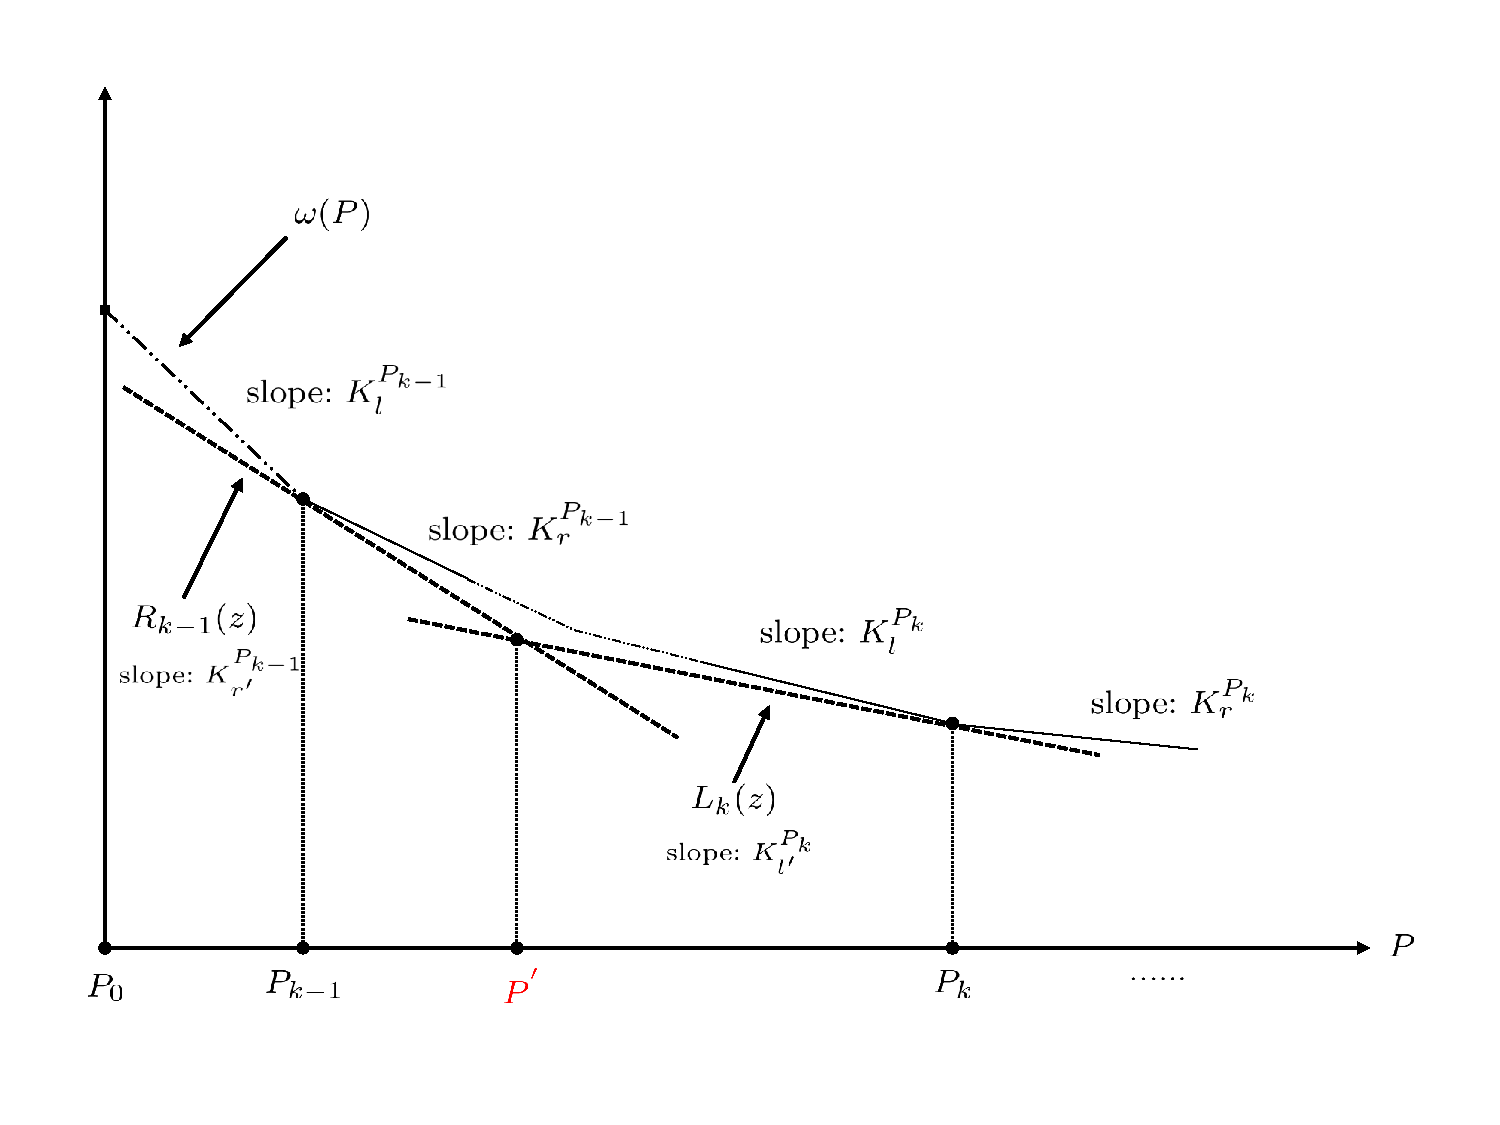
\includegraphics[width=0.95\textwidth]{Figures/IPC}
	\end{figure}
	\centering
\end{frame}


\begin{frame}{CP Algorithm}
	The Cutting Plane(CP) Algorithm to compute $\omega(P)$ for a given $P$.
	\begin{description}
	  \justifying
		\footnotesize
	  \item[Step 1.] Let $\mathbb{S}'\subseteq \mathbb{S}\setminus \{N\}$ indicates a restricted coalition set, which includes some initial coalitions,
	  \vspace{10pt}
	  e.g.,$ \{1\},\{2\},\ldots,\{v\}$.
	  \item[Step 2.] Find an optimal solution $\bar{\alpha}(\ \cdot \ ,P)$ to LP $\tau(P)$:
	  \begin{equation*}
	  \max_{\alpha\in \mathbb{R}^n} \big\{ \alpha(N,P): \alpha(s,P) \leq c(s)+P, \mbox{ for all } s \in \mathbb{S}'\big\}.
	  \end{equation*}
	  \vspace{-11pt}
	  \item[Step 3.]
	  Find an optimal solution $s^*$ to \textcolor{red}{the separation problem}:
	  \begin{equation*}
	  \delta = \min \big\{ c(s)+ P -\bar{\alpha}(s,z): \forall s \in \mathbb{S} \setminus \{N\}\big\}.
	  \end{equation*}
	  \item[Step 4.]
	  If $\delta<0$, then add $s^*$ to $\mathbb{S}'$, and go to step 2; otherwise, return $\omega(P)=c(N)-\bar{\alpha}(N,P)$.
	\end{description}

\end{frame}


\begin{frame}{DP Algorithm}
	The Dynamic Programming(DP) Algorithm to solve the separation problem.
	\begin{description}
	\justifying
	\footnotesize
	\item[Step 1.] Initially, let $D(k,u)$ indicate the minimum objective value of the restricted problem of separation problem, where $k\in \{1,2,\ldots,v\}$ and $u\in \{0,1,\ldots,v\}$.
	\item[Step 2.] Given the initial conditions $D(1,0) = P$ and $D(1,1) = t_1 - \beta_1 +P$. The boundary conditions are $D(k,u) = \infinity$ if $u > k$, for all $k \in V$.
	\item[Step 3.] Given the recursion:
	\begin{equation*}
	D(k,u)= \min \left\{
	\begin{aligned}
	& D(k-1,u), \text{for the case when} \ s^* \ \text{does not contain} \ k, \\
	& D(k-1,u-1) + u t_k - \alpha_k ,\text{for the case when} \ s^* \ \text{contains} \ k.
	\end{aligned}
	\right.
	\end{equation*}

\item[Step 4.] Obtain the optimal objective value of separation problem by
$\delta_{AIPU} = \min\{D(v,u): u\in \{1,2,\ldots,v-1\}\}$.
 return $\delta_{AIPU}$.
	\end{description}

\end{frame}

\begin{frame}{Computational Results}
	\vspace{-3mm}
	\begin{figure}[H]
	\centering
	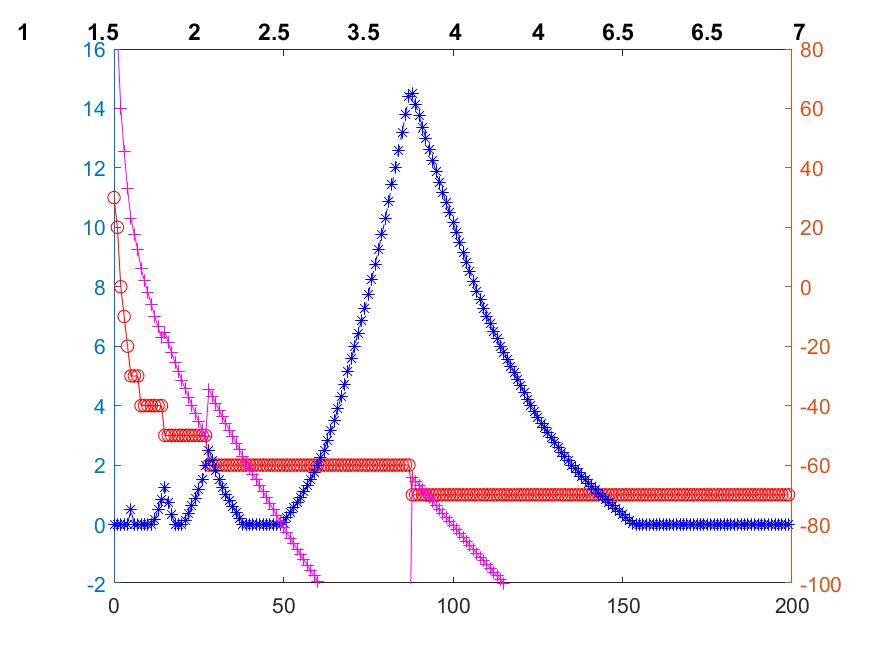
\includegraphics[width=0.95\textwidth]{Figures/Image30}
	\end{figure}
	\centering
\end{frame}

\section{Extension and Generalization}
\begin{frame}
\centering
\large
\textcolor{blue}{\bf {\huge E}XTENSION \&  {\huge G}ENERALIZATION}
\end{frame}

\begin{frame}{Machine Scheduling Game with Weighted Jobs}
	\begin{itemize}
	\justifying
		\item Each job $k \in V$ has a processing time and a weight denoted by $t_k,\omega_k$, respectively.
		\vspace{2pt}
		\item $c(S)$ can be obtained by assuming that\\
		\quad $t_1/\omega_1 \leq t_2/\omega_2 \leq \ldots \leq t_v/\omega_v$.
		\vspace{2pt}
		\item $P_m = c_0(V,m)- c_0(V,m-1), 2 \leq m \leq v$.
		\item ${\omega(P)}$ is piecewise linear, and convex in price $P$ at each subinterval.
		\vspace{2pt}
		\item The separation problem can be solved in polynomial time.
\end{itemize}
\end{frame}

\begin{frame}{Pricing in General IM Games}
	\begin{itemize}
	\justifying
		\item \textcolor{red}{$ILP:$}
		$c(S,m(S,P))= \mathop{\min}_{x} \{ cx+Pm(x): Ax \geq By^s+D, \tilde{\alpha}x \leq m, x \in \mathbb{Z}^{t \times 1} \}$
		\vspace{2pt}
		\item \textcolor{blue}{Decompose} $c(S,m(S,P))$ into $\textcolor{blue}{c_0(S,m(S))}+Pm.$
		\vspace{2pt}
		\item $c_0(V,m)- c_0(V,m-1) > 0 \Leftrightarrow P_m > 0, m=2,\ldots,v.$
		\item $c_0 (V,m) - c_0 (V,m+1) < c_0 (V,m-1) - c_0 (V,m) \Leftrightarrow \quad P_m < P_{m+1} , m=2,3,\ldots,v-1.$
		\vspace{3pt}
		\footnotesize
		\item $c_0(S_1,m-1)-c_0(S_1,m) \geq
  c_0(S_1,m)-c_0(S_1,m+1) \quad m=2,\ldots,v-1.$
		\item $	c_0(S_1,m-1)-c_0(S_1,m) \leq
	  c_0(S_2,m-1)-c_0(S_2,m) \\
		\quad \quad m=2,\ldots,v$, where ~$S_1 \subset S_2$.
	\end{itemize}
\end{frame}

\section{Conclusion}
\begin{frame}{Conclusions}
\centering
\large
\vspace{1mm}
\textcolor{blue}{\bf {\huge C}ONCLUSIONS}
\vspace{2mm}
\begin{itemize}
\normalsize
\justifying
\item[$\star$] \textcolor{purple}{Cooperative Game Theory}:
\begin{itemize}
\small
\vspace{2mm}
\item[$-$] {New Instrument for Stabilization via Setup cost Pricing}.
\vspace{2mm}
\end{itemize}
\item[$\star$] \textcolor{purple}{Scheduling Problem}:
\begin{itemize}
\small
\vspace{2mm}
\item[$-$] Parallel Machine Scheduling with Setup Cost.
\vspace{2mm}
\end{itemize}
\item[$\star$] \textcolor{purple}{Models, Solution Methods and Applications}:
\begin{itemize}
\small
\vspace{2mm}
\item[$-$] Several ILP formulations;
\vspace{2mm}
\item[$-$] Cutting Plane to solve the seperation problem;
\vspace{2mm}
\item[$-$] Implementations on the MSGW game.
\end{itemize}
\end{itemize}
\end{frame}

\begin{frame}{The End}
\begin{center}
	\begin{LARGE}
		Thank you!
	\end{LARGE}
\end{center}
\end{frame}
\end{document}
